\documentclass{article}

\makeatletter
\def\input@path{{neurips_style_files/}}
\makeatother
\usepackage[preprint]{neurips_2024}

\usepackage[utf8]{inputenc}
\usepackage[T1]{fontenc}
\usepackage{hyperref}
\usepackage{url}
\usepackage{booktabs}
\usepackage{amsfonts}
\usepackage{amsmath}
\usepackage{microtype}
\usepackage{xcolor}
\usepackage{graphicx}
\usepackage{multirow}
\usepackage{array}
\usepackage{verbatim}

\title{Evaluating Hallucination Direction Ablation for Truthfulness: Orthogonal-Style Suppressive Patching, Baseline Comparison, and Route Pivot on TruthfulQA}

\author{
  Lingyun Chen \\
  \texttt{lchen47@ncsu.edu}
}

\begin{document}
\maketitle

\begin{abstract}
This report evaluates a proposal-consistent \emph{hallucination direction ablation} (HDA) patch as one route for truthfulness improvement on \texttt{Qwen/Qwen3-4B-Instruct-2507}, and compares it against an external factuality baseline and a stronger internal reranking route. We implement an end-to-end stack for source-locked TruthfulQA preparation, deterministic binary evaluation, task-aligned direction extraction, activation intervention, and rank-one directional patching, with orthogonal projection as the $\alpha = 1$ special case and tuned suppressive patching as the final operating point. The HDA route delivers a stable but modest gain: the chosen canonical operating point (\texttt{MLP layers 18--19}, $\alpha=2.8$) improves TruthfulQA binary accuracy by \textbf{+0.97 points on average across 10 held-out seeds}, with \textbf{10/10 positive seeds}, while a neighboring narrow late-MLP configuration remains competitive. On a lightweight paired regression package, the same 4B patch shows \textbf{no measured regression} on the HellaSwag / MMLU-slice / GSM8K probes and only \textbf{2\% material drift} on 100 benign prompts. However, stronger gains come from a route pivot: a fixed factual verifier reranking method improves TruthfulQA by \textbf{+2.37 points across 6 seeds} on the standardized shared-seed comparison. We also add \textbf{DoLa} as a recognized external factuality baseline from prior work. Under a decode-compatible A/B generation proxy, DoLa did not outperform the base model, and \texttt{HDA + DoLa} showed no additive gain over HDA alone. A binary-to-open bridge on 40 matched questions did not show stronger open-generation support for the patched model, so the HDA result should be read as \textbf{proxy-limited evidence} rather than as a validated free-form truthfulness gain. Cross-model tests show partial portability to \texttt{Qwen3-1.7B}, \texttt{Qwen3-0.6B}, and \texttt{Llama-3.2-1B}, but only the 4B setting preserves a clean truthfulness--stability tradeoff; this should be read as a boundary result rather than a strong portability claim. Github code link: \url{https://github.com/Franklyc/Hallucination-Direction-Ablation}.
\end{abstract}

\section{Introduction}
Hallucination remains a central deployment failure mode for large language models: the model produces fluent but false or weakly grounded answers, often in exactly the settings where users most want reliability. TruthfulQA was explicitly designed to expose this gap and shows that scaling alone does not guarantee improved truthfulness \citep{lin-etal-2022-truthfulqa}. In practice, many mitigation methods trade one problem for another: decoding-time control adds integration complexity, sampling-heavy verification raises latency, retrieval is unavailable in many deployment settings, and aggressive editing can distort ordinary outputs.

This project began from a narrow mechanistic question: can a \emph{training-free directional patch} suppress a hallucination-related direction in model internals and yield measurable truthfulness improvement without retraining? The original proposal was aligned with recent mechanistic steering and intervention work \citep{li2024iti,arditi2024refusal}: estimate a direction from calibration data, then orthogonalize selected write matrices so the model writes less into that direction. In the final paper, we keep that orthogonal-projection intuition as the conceptual starting point and $\alpha = 1$ special case, but treat the deployed method more generally as a rank-one suppressive directional edit. This route is appealing because it is lightweight, parameter-efficient, and deployment-friendly: once patched, the model can be used with standard decoding and no runtime intervention logic.

As the project progressed, the evaluation surfaced three realities. First, HDA does work, but the effect is small and sensitive to where the patch is applied. Second, the strongest empirical gains in this codebase come from a different route: verifier reranking. Third, the binary ranking gain does not automatically transfer to better open-generation support on a matched bridge set. The final report therefore keeps both views in scope. It treats HDA as the main proposal-consistent method and verifier reranking as the strongest internal empirical route, while treating the bridge result as a limit on how far the HDA claim should travel. Accordingly, the report is structured as a route comparison with asymmetric roles: HDA is the main proposal-consistent intervention, verifier reranking is the strongest empirical route, and DoLa is the external prior-method baseline. This framing matches the course requirement to both pursue a motivated new method and compare against established baselines and alternative routes.

The final contribution is therefore not a single oversized claim. Instead, it is a careful empirical answer to four questions:
\begin{itemize}
\item Can a proposal-consistent suppressive directional HDA patch produce stable truthfulness gains on the main model?
\item Does the patch avoid measured regression on a lightweight paired regression package?
\item How does HDA compare with an established external factuality baseline such as DoLa?
\item How portable is the patching idea across smaller models and another model family?
\end{itemize}

\section{Method}
\subsection{TruthfulQA Binary Protocol}
The main benchmark is a deterministic binary version of TruthfulQA built from the public multiple-choice source rows \citep{lin-etal-2022-truthfulqa}. For each question, we take the row's \texttt{Best Answer} as the truthful candidate and \texttt{Best Incorrect Answer} as the unsupported candidate. The final evaluator does \emph{not} resample from the larger lists of alternative correct or incorrect answers: the candidate texts are fixed once the source row is chosen. What changes with the split seed is only the calibration/evaluation partition and the A/B ordering of the two fixed candidate texts. Under a fixed prompt template, the model prediction is the higher-scored option:
\[
\hat{y}(q) = \arg\max_{a \in \{a_{\text{true}}, a_{\text{false}}\}} \log P(a \mid q, \text{prompt}).
\]
The prompt always asks for a single-letter answer (\texttt{A} or \texttt{B}), and the A/B order is assigned by a deterministic per-question RNG derived from the split seed. This log-probability protocol is the main reporting standard throughout the project because it removes decoding variance and supports paired comparisons question-by-question. At the same time, it should be read as a \emph{ranking-style truthfulness proxy}, not as a full free-form hallucination benchmark: a model that cleanly ranks two fixed candidates need not behave identically in open-ended generation.

\subsection{Task-Aligned HDA Direction Extraction}
The calibration split is used to estimate layer-wise task-aligned contrastive directions associated with truthful versus unsupported behavior. At a high level, the direction is computed from contrastive activation differences between prompt variants designed to encourage correct factual behavior versus overconfident unsupported behavior. For each layer $\ell$, we obtain a direction vector $\hat{v}_\ell$ and then evaluate whether suppressing that direction improves held-out truthfulness. We do not interpret this direction as a universal hallucination axis; rather, it is a task-aligned intervention target for this benchmark and prompting setup.

\subsection{Rank-One Directional Suppression Patch}
The permanent HDA patch edits selected write matrices with a rank-one directional update:
\[
W' = W - \alpha \hat{v}_\ell (\hat{v}_\ell^\top W),
\]
where $\alpha$ is the patch strength. When $\alpha = 1$, this corresponds to the clean ``remove the write component along $\hat{v}_\ell$'' intuition of a rank-one orthogonal projector. Our best setting, however, is $\alpha = 2.8$, which is \emph{not} a pure orthogonalization constant. Geometrically, it is better understood as an \emph{over-subtractive suppression coefficient}: the edit first cancels the write component along the extracted direction and then pushes the selected write slightly past zero along that axis. In that sense, the best patch behaves less like ``neutralize one axis'' and more like ``apply a stronger penalty along a harmful axis until the residual write no longer wins.'' We do \emph{not} read this as evidence that the model contains a clean opposite ``truth direction'' that we have recovered; the safer interpretation is simply that nulling the extracted direction is insufficient, while a slightly stronger suppressive edit works better on this benchmark. Accordingly, ``orthogonal patch'' in this report should be read as the conceptual $\alpha = 1$ starting point of the update family, while the final deployed method is a tuned suppressive directional variant of the same rank-one edit. This is a training-free parameter edit: it does not add runtime hooks, extra forward passes, or new learned parameters. The key design degrees of freedom are:
\begin{itemize}
\item \textbf{Layer range}: which layers are patched;
\item \textbf{Module choice}: attention output, MLP output, or both;
\item \textbf{Strength}: the suppression coefficient $\alpha$.
\end{itemize}

\subsection{Verifier Reranking Route}
Although the project proposal focused on HDA, the codebase also developed a verifier reranking route. It scores each candidate answer with a factual verifier prompt and selects the candidate with the better factuality margin. This route is still lightweight and training-free, but unlike HDA it adds a separate scoring stage at inference time, conceptually placing it closer to verification-style methods than to permanent parameter editing \citep{manakul-etal-2023-selfcheckgpt}.

\subsection{DoLa Baseline and HDA + DoLa}
To satisfy the final-stage comparison requirement, we add DoLa as an external prior-method baseline aimed at factuality improvement. Because DoLa is a decode-time method, it cannot be inserted into the original sequence-logprob scorer. We therefore evaluate it through a compatible A/B \emph{generation proxy}: the same binary question is shown to the model, but the model is asked to generate either \texttt{A} or \texttt{B} greedily. This keeps the task and prompt nearly identical while allowing decode-time logic to operate. However, this proxy is also structurally unfavorable to DoLa: the candidate space is collapsed to a one-token decision, so layer-contrastive decoding has much less sequence structure to exploit than in its intended multi-token generation regime. We test a clean $2 \times 2$ matrix:
\begin{itemize}
\item Base
\item Base + DoLa
\item HDA patch
\item HDA patch + DoLa
\end{itemize}
and interpret the result cautiously as a baseline comparison under a decode-compatible proxy rather than as a replacement for the main logprob protocol. This comparison is informative but not strictly protocol-equivalent to the main log-prob evaluation, so it should be read as a constrained baseline check rather than a definitive method ranking.

\subsection{Paired Regression Package}
The final evaluation package is intentionally small and reproducible. For a fixed patched model, it runs:
\begin{itemize}
\item TruthfulQA binary (full held-out set),
\item HellaSwag validation slice ($n=500$),
\item MMLU representative slice ($6$ subjects $\times 50 = 300$),
\item GSM8K slice ($n=200$),
\item a benign drift set.
\end{itemize}
The benign drift set contains $n=100$ prompts with five equally sized families ($20$ each): summarization, rewriting, extraction, formatting, and simple transformation / short-answer tasks. This 100-prompt benign set is a fixed project-side evaluation list released with the repository so the paired drift check can be rerun unchanged. Drift similarity is reported as the mean cosine similarity between sentence embeddings from \texttt{sentence-transformers/all-MiniLM-L6-v2}. We flag \emph{material drift} if the cosine similarity falls below $0.85$, if refusal status flips, if format-pass status flips, or if the patched/base output-length ratio falls outside $[0.5, 1.5]$. This package answers the central deployment question: does the patch improve the target metric without obviously damaging unrelated behavior? It should be interpreted as a \emph{regression canary}, not as a benchmark with enough power to rule out every sub-1-point non-target change. In particular, these slices are not powered to exclude regressions on the same order as the HDA gain itself; they are meant to catch visible collateral damage, not to certify full capability preservation.

\section{Dataset and Processing}
\subsection{TruthfulQA Split Construction}
The project uses the TruthfulQA multiple-choice source set and converts it into the deterministic binary format above. Each binary item therefore always uses the same source-row question text, the same \texttt{Best Answer}, and the same \texttt{Best Incorrect Answer}; only the A/B placement of those two candidate strings varies with the split seed. The split protocol itself always has the same form:
\begin{itemize}
\item \textbf{Calibration}: 200 questions, used for direction extraction and configuration selection;
\item \textbf{Held-out evaluation}: 590 questions, used for final reporting only.
\end{itemize}
Two evaluation views are reported. First, a \emph{canonical} seed-41 split is used for detailed paired regression, example-level comparisons, and the main table entries that require one concrete held-out set. Seed 41 was designated in advance as the single canonical split for detailed analysis before the final multiseed robustness expansion; it was not chosen post hoc because it looked favorable. Second, the reported multi-seed HDA and verifier summaries average over repeated seed-indexed stratified 200/590 partitions of the same form. In those summaries, ``held-out'' refers to the 590-question evaluation portion of each seed-specific split, not to a single universal set shared by every number in the paper. Once a particular split seed is fixed, the scorer itself is deterministic; the seed variation reflects repeated split construction and candidate ordering rather than stochastic decoding.

Configuration selection is also fixed relative to that split protocol. For the main Qwen3-4B HDA result, the final layer range, module choice, and $\alpha$ were selected once on the canonical 200-question calibration split, then frozen before the 10-seed expansion. We did \emph{not} re-tune a separate patch for each seed-specific split. The final report also includes simpler controls---for example $\alpha=1$ on the same layer band and broader all-layer edits---to reduce the risk that the reported gain is explained only by broad intervention or by a single uncontextualized tuned configuration.

\begin{figure}[t]
  \centering
  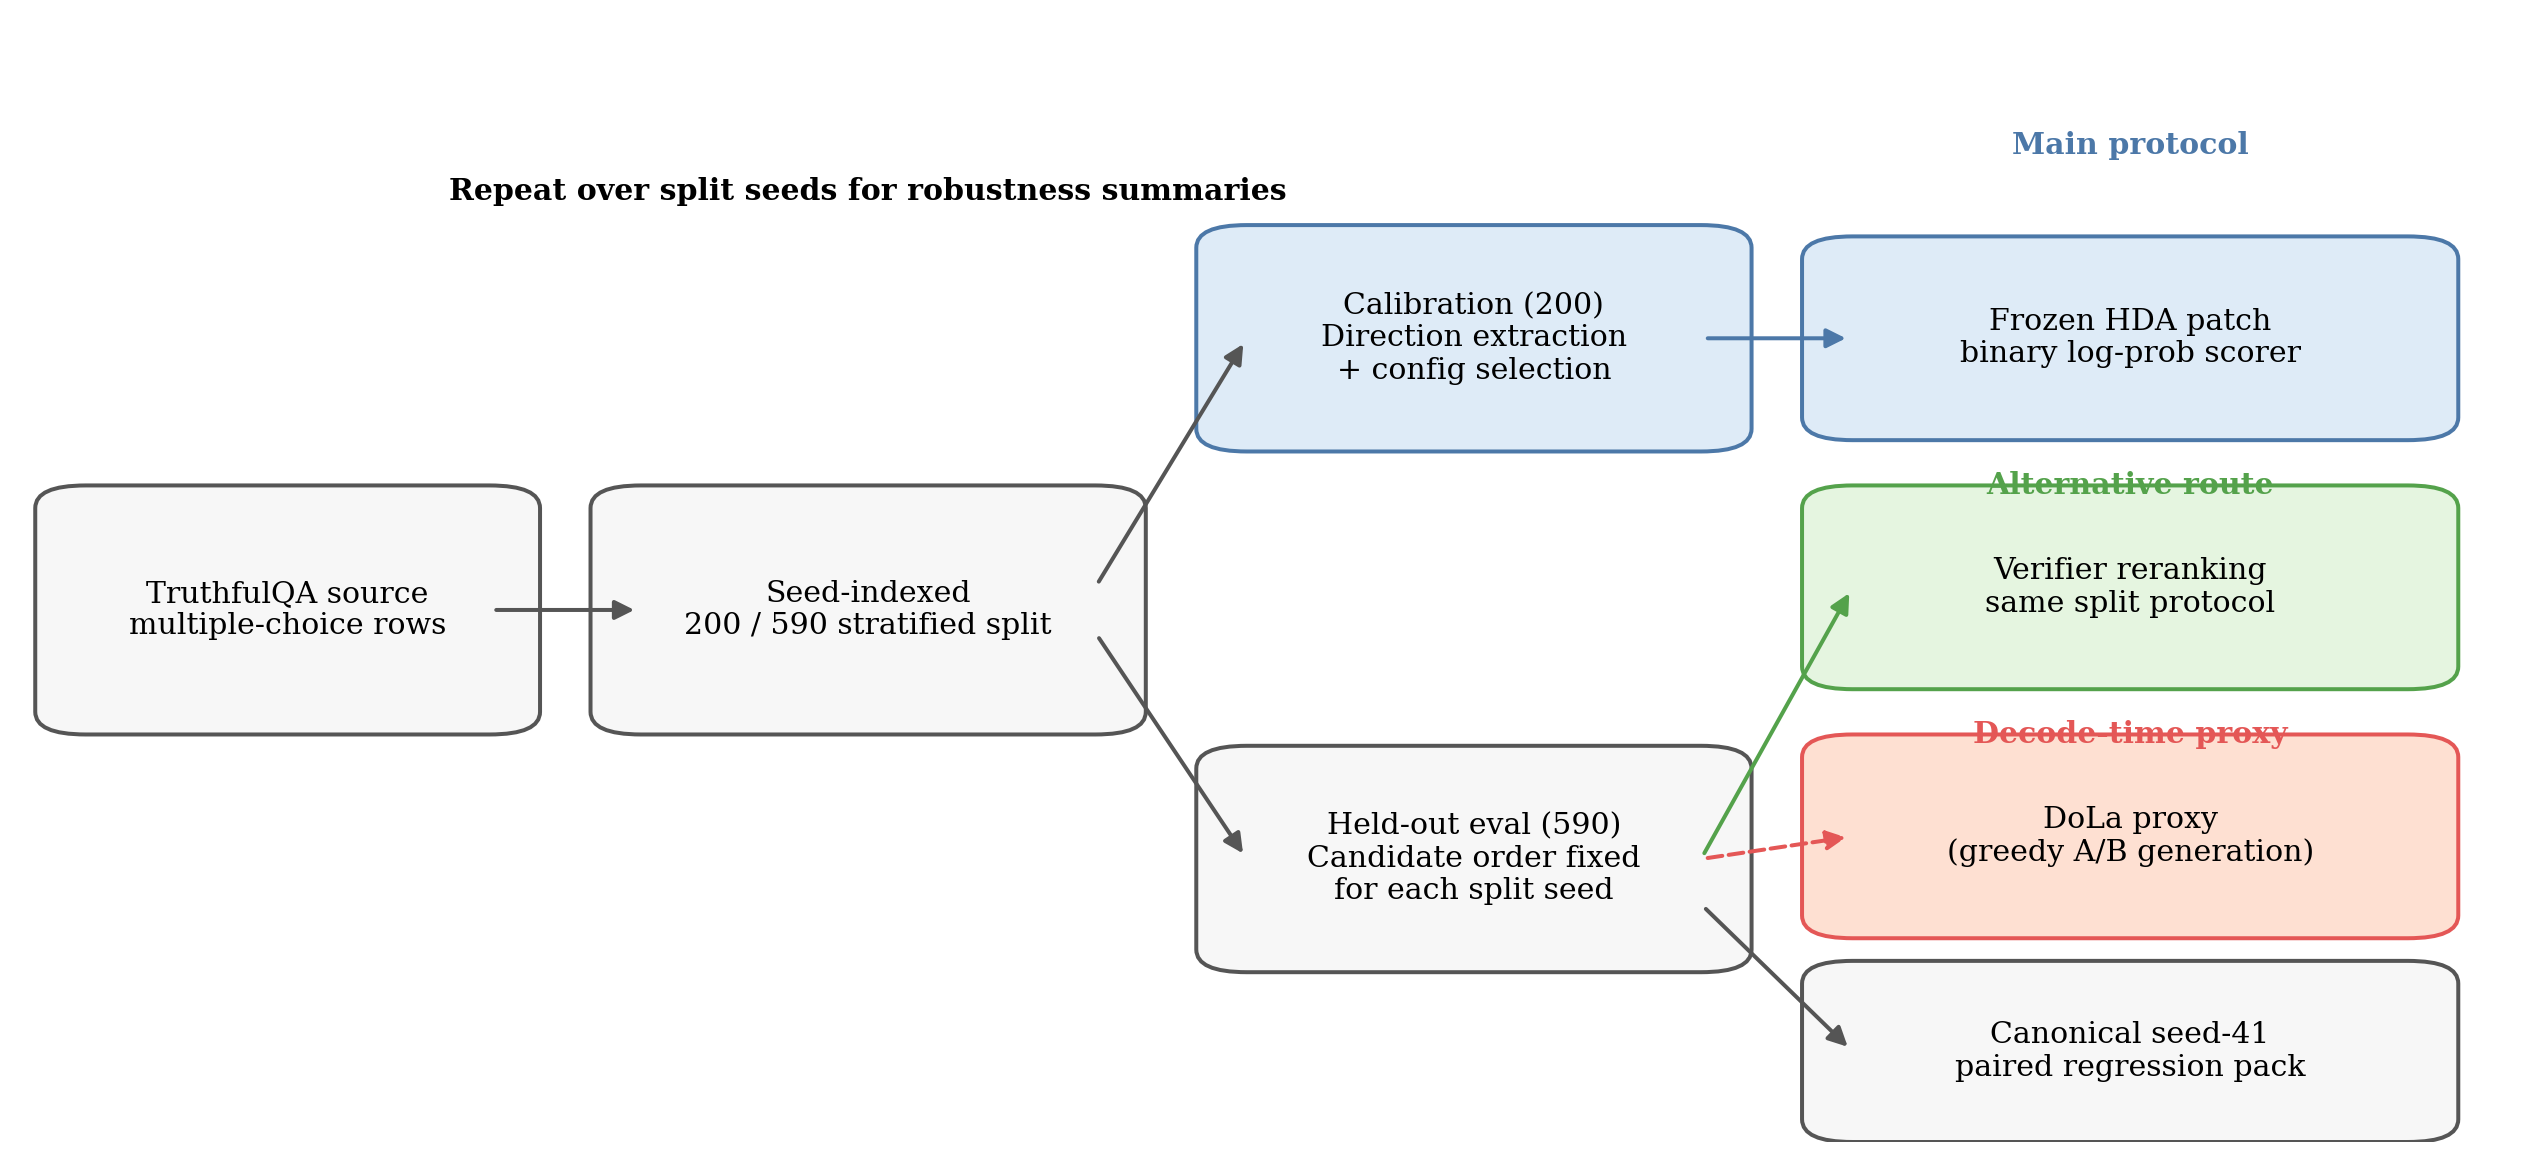
\includegraphics[width=\linewidth]{experiments/artifacts/route_plots/final_protocol_schematic.png}
  \caption{Evaluation protocol schematic. The main HDA and verifier results use the binary log-probability protocol over repeated seed-indexed 200/590 splits, while DoLa is evaluated only through a separate greedy A/B generation proxy. The paired regression package is reported on the canonical seed-41 split.}
  \label{fig:protocol}
\end{figure}

\subsection{Regression and Drift Data}
The paired regression package uses lightweight held-out slices rather than full public leaderboards. This is a deliberate tradeoff: the goal is not a full capability audit, but a regression pack that can be run repeatedly during model editing. Specifically, we use HellaSwag validation $n=500$, an MMLU slice of six subjects with 50 questions each ($n=300$; \texttt{high\_school\_biology}, \texttt{high\_school\_us\_history}, \texttt{college\_computer\_science}, \texttt{formal\_logic}, \texttt{business\_ethics}, \texttt{high\_school\_macroeconomics}), GSM8K $n=200$, and a benign drift set of $n=100$ prompts. Benign drift is measured by mean embedding cosine, exact-match rate where applicable, output-length ratio, refusal-rate change, format-pass change, and the material-drift rule defined above.

\subsection{Qwen3 Thinking-Mode Handling}
An important methodological issue emerged for smaller Qwen3 models. \texttt{Qwen3-1.7B} and \texttt{Qwen3-0.6B} are hybrid reasoning models. Under the default reasoning mode, the binary evaluator collapsed into an ``always A'' behavior. In our setup, the main cause is the default reasoning preamble: these models try to begin with a \texttt{<think>} segment before producing the final answer token, while our evaluator expects the first scored answer token to be the one-letter decision itself. Hard-disabling thinking fixed the evaluator and made patch experiments meaningful. This alignment step is also methodologically reasonable for this project, because the main target model is \texttt{Qwen3-4B-Instruct-2507}, an instruct model used in short-answer mode rather than in explicit CoT mode. The non-thinking setting therefore makes the 1.7B and 0.6B evaluations better matched to the main-model protocol instead of leaving them in a mismatched reasoning-template regime.

\section{Results}
\subsection{Main Qwen3-4B HDA Result}
Table~\ref{tab:qwen4b-main} summarizes the main Qwen3-4B results. The chosen canonical HDA configuration patches the \texttt{MLP} write matrices at layers 18--19 with $\alpha=2.8$. This yields \textbf{+0.97 TruthfulQA points on average across 10 held-out split seeds}, with \textbf{10/10 seeds positive}. Here, the 10-seed summary means 10 repeated 200/590 stratified split constructions under an otherwise deterministic evaluator, with the patch configuration frozen in advance. The corresponding two-sided exact sign test for 10/10 positive split deltas is $p=0.00195$. A neighboring narrow late-MLP patch on layers 18--20 reaches a nearly identical regression-checked result, so the evidence supports a \emph{narrow late-MLP family} more strongly than an exact unique-band discovery; the 18--19 setting is kept as the canonical operating point by parsimony. On the canonical split, the tuned patch changes 11 of 590 item-level decisions: it fixes 9 and breaks 2, for a net gain of 7 items. The corresponding exact McNemar / sign test on the discordant pairs gives $p=0.065$, so the strongest evidence comes from the combination of paired bootstrap support and the 10/10 split-seed sign consistency rather than from a single-split significance threshold. This is therefore best read as a \emph{small but repeatable} effect, not as a large deployment jump: in practical terms, the permanent patch moves only a handful of canonical-split decisions, and verifier reranking remains the more consequential route when latency is acceptable. On the paired regression pack, the same patched model shows no measured regression on the small HellaSwag, MMLU-slice, and GSM8K probes, while benign drift remains limited (\textbf{0.974} mean similarity, \textbf{2\%} material drift).

\begin{table}[t]
\centering
\caption{Main Qwen3-4B results on TruthfulQA and the paired regression package. TruthfulQA accuracy and regression rows use the canonical seed-41 split; the multiseed delta row reports robustness over repeated 200/590 split seeds with the configuration frozen in advance.}
\label{tab:qwen4b-main}
\begin{tabular}{lcc}
\toprule
\textbf{Metric} & \textbf{Base} & \textbf{Patched / Delta} \\
\midrule
TruthfulQA binary accuracy (canonical split) & 77.97\% & 79.15\% \\
TruthfulQA paired bootstrap CI (canonical split) & -- & [\textbf{+0.17}, \textbf{+2.37}] points \\
TruthfulQA multiseed robustness delta & -- & \textbf{+0.97 points} (10 seeds, 10/10 positive) \\
HellaSwag slice ($n=500$) & 33.8\% & +0.2 points \\
MMLU slice ($n=300$) & 67.67\% & +0.33 points \\
GSM8K slice ($n=200$) & 78.5\% & +0.5 points \\
Benign drift similarity ($n=100$) & 1.000 & 0.974 \\
Benign material drift rate ($n=100$) & 0.00 & 0.02 \\
\bottomrule
\end{tabular}
\end{table}
For the non-target regression slices, we do not interpret the small positive deltas as evidence of capability gains. The paired bootstrap intervals are HellaSwag $[-0.8, +1.2]$ points, MMLU-slice $[-0.67, +1.67]$ points, and GSM8K $[-2.0, +3.0]$ points. All three lightweight non-target intervals cross zero; the claim is only that this small regression pack did not measure an obvious regression for the main Qwen3-4B patch.

\begin{figure}[t]
  \centering
  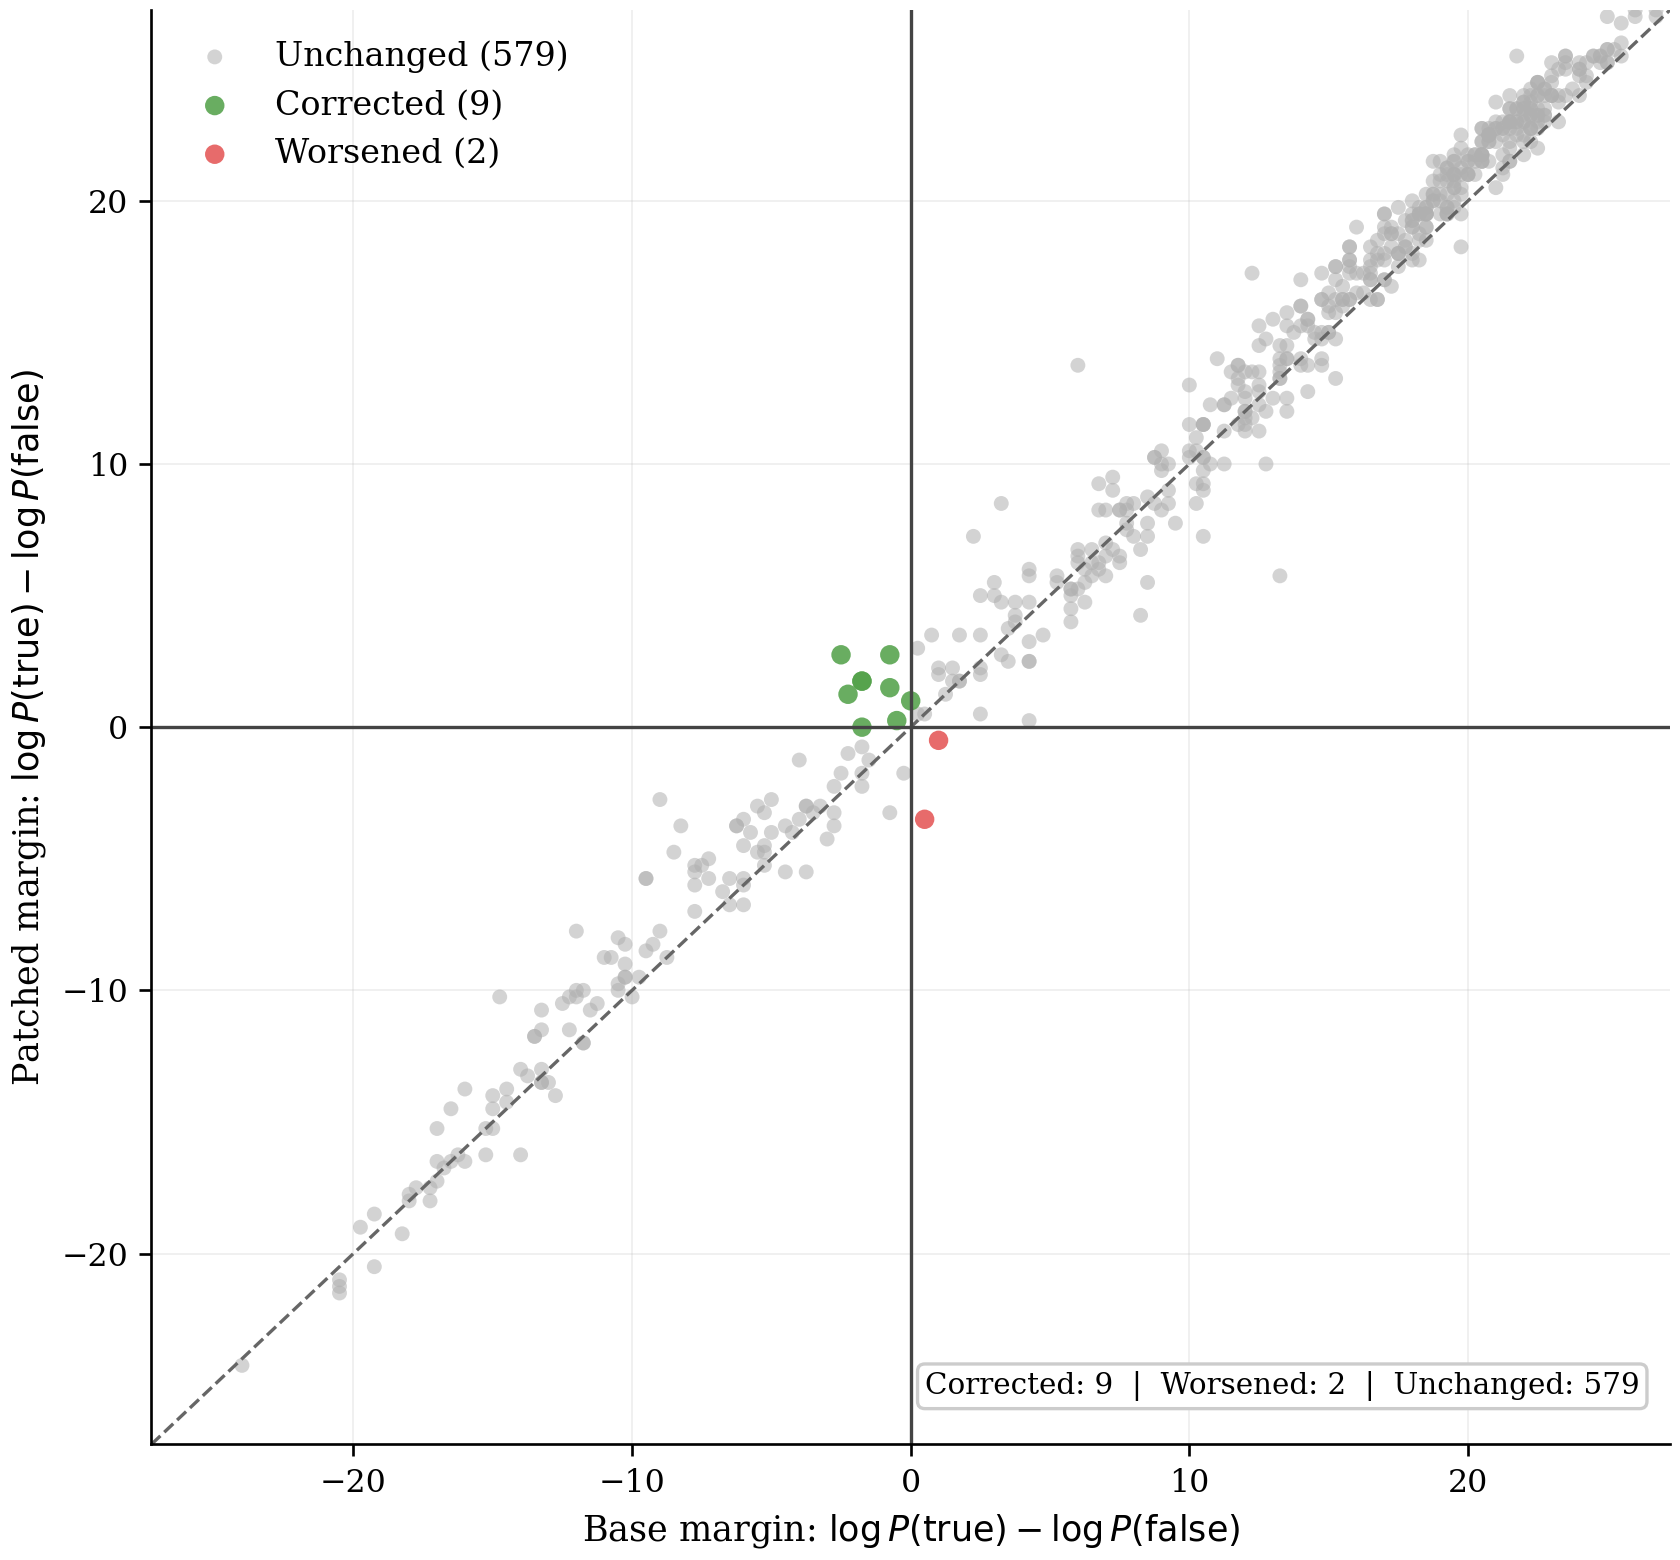
\includegraphics[width=0.78\linewidth]{experiments/artifacts/route_plots/final_qwen4b_margin_shift.png}
  \caption{Per-question margin shift for the tuned Qwen3-4B patch on the canonical split. Most points stay near the diagonal, showing that the patch mostly nudges existing margins rather than broadly rewriting behavior; only 11 items flip, with 9 corrected and 2 worsened.}
  \label{fig:margin-shift}
\end{figure}

\subsection{Was the Original ``Orthogonal'' Idea Enough?}
The original proposal concept was a clean orthogonal special case, corresponding roughly to $\alpha = 1$. Final controls show that this was \emph{not} the best operating point. On the same key layer band, $\alpha=1$ only gives \textbf{+0.34} points on Qwen3-4B, far below the tuned $\alpha=2.8$ result. Broadening the patch to all MLP layers with $\alpha=1$ shrinks the gain further to \textbf{+0.17} points, and an all-layer \texttt{both}-module control turns negative on a 180-item subset. The conclusion is clear: HDA helps only when it is \emph{surgically placed}. The useful intervention is not ``apply the same suppressive edit everywhere,'' but ``apply a narrow directional suppression patch to the write region that actually carries the harmful signal.'' Figure~\ref{fig:hda-heatmap} makes this structural point explicit: narrow MLP edits become positive, while broader or differently targeted edits do not.

\begin{figure}[t]
  \centering
  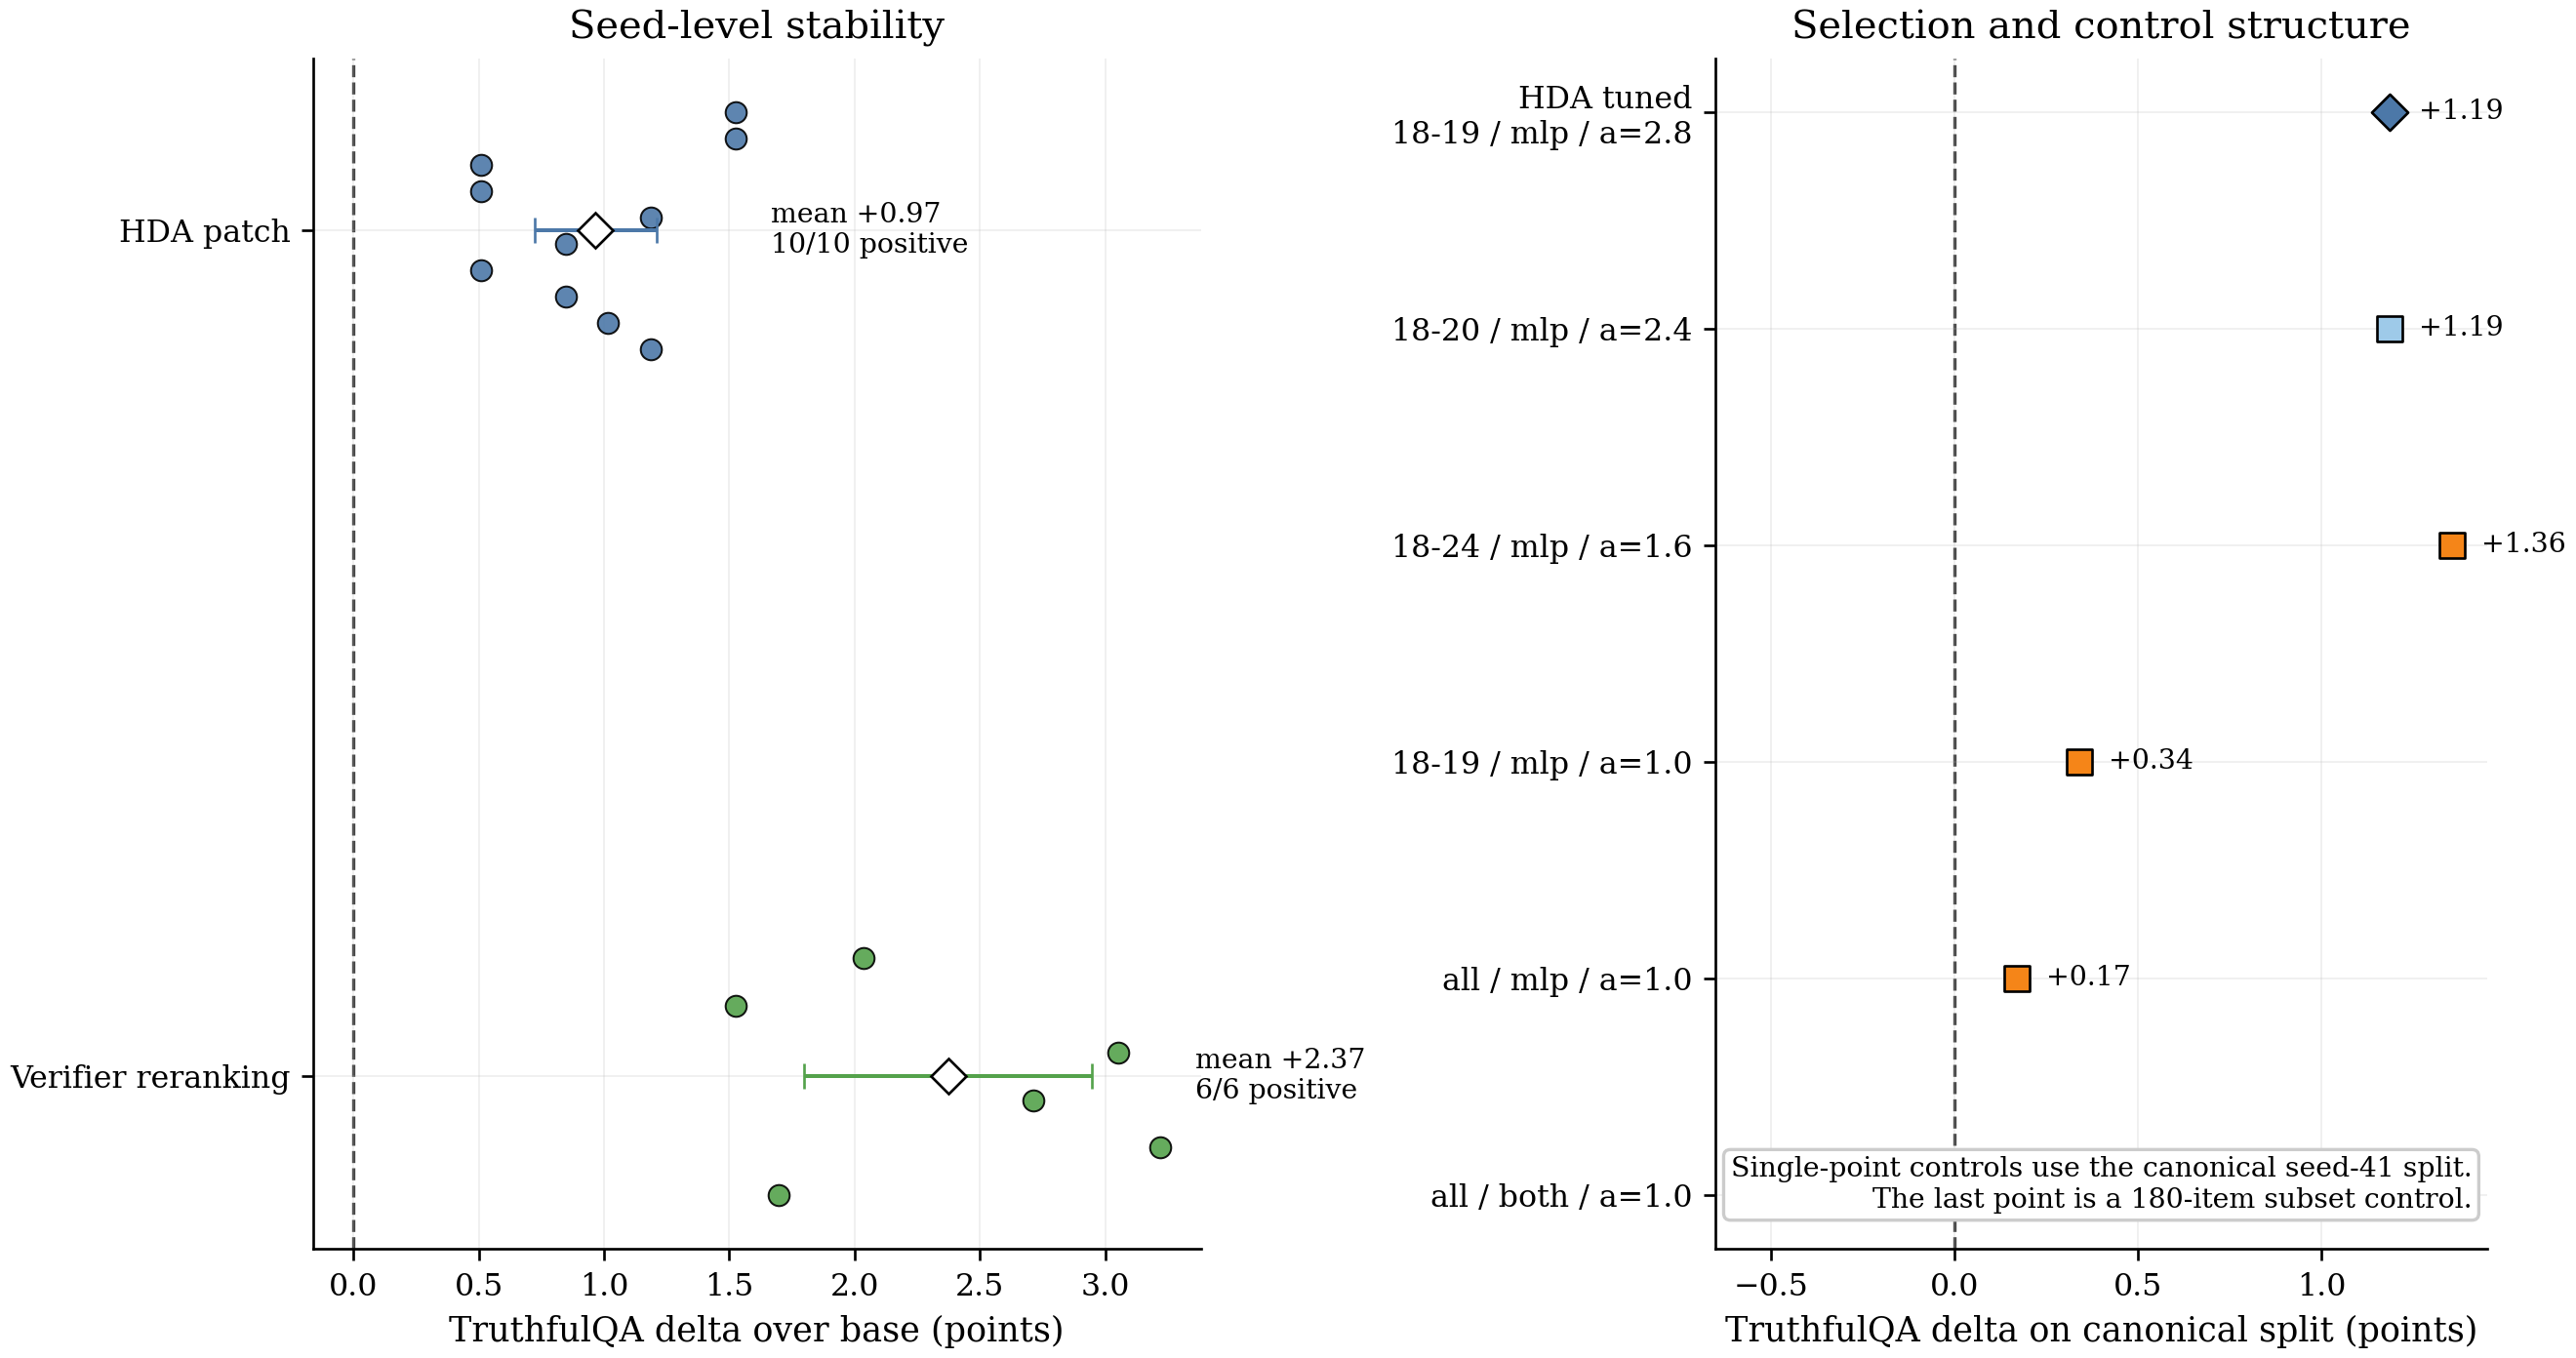
\includegraphics[width=\linewidth]{experiments/artifacts/route_plots/final_qwen4b_route_delta.png}
  \caption{Main Qwen3-4B route comparison and patch controls under the original binary log-probability protocol. The left panel shows seed-level stability for HDA and verifier; the right panel shows canonical-split control configurations. The tuned HDA patch is stable but modest, while verifier reranking is much stronger.}
  \label{fig:qwen4b-routes}
\end{figure}

\begin{figure}[t]
  \centering
  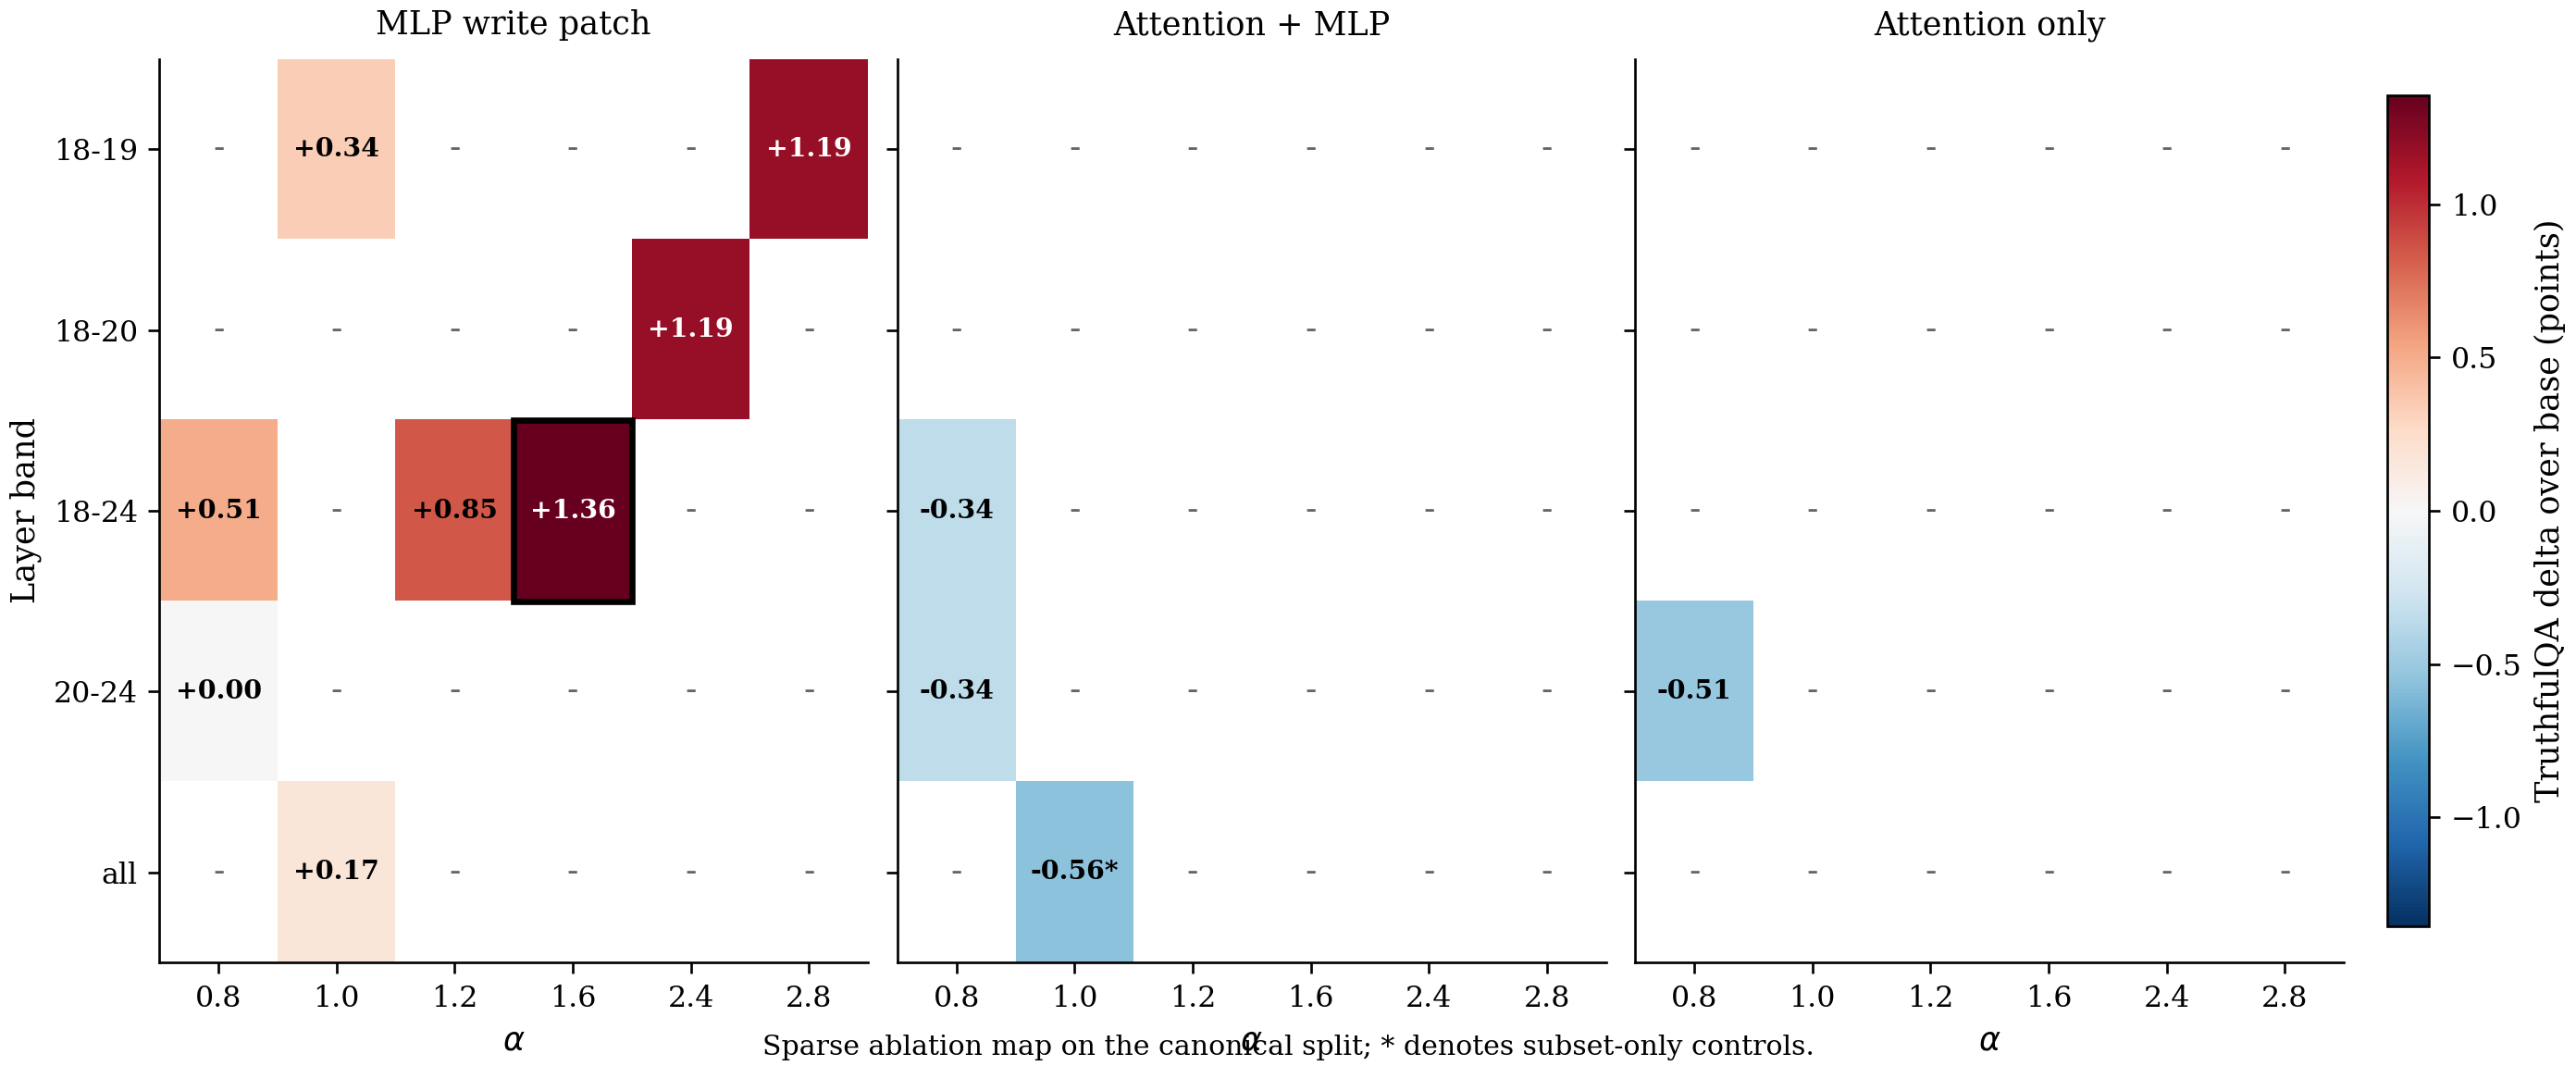
\includegraphics[width=\linewidth]{experiments/artifacts/route_plots/final_hda_ablation_heatmap.png}
  \caption{Sparse HDA ablation map on the canonical split. Positive results concentrate in narrow MLP edits around layers 18--20, while broader or differently targeted controls weaken or reverse the gain. The black box marks the selected operating point used for the main multiseed result.}
  \label{fig:hda-heatmap}
\end{figure}

\subsection{External Baseline Comparison: DoLa}
DoLa was added as a recognized prior-method baseline aimed specifically at factuality improvement \citep{chuang2024dola}. Under the decode-compatible A/B generation proxy on Qwen3-4B:
\begin{itemize}
\item Base: 78.31\%
\item DoLa: 77.97\%
\item HDA: 78.81\%
\item HDA + DoLa: 78.81\%
\end{itemize}
Two conclusions follow. First, under this proxy, DoLa did not outperform the base model. Second, under the same proxy, combining DoLa with the tuned HDA patch yielded \emph{no additive gain} over HDA alone. The most likely interpretation is that the two methods are partially redundant in this regime: both aim to suppress misleading higher-layer signals, so the combination does not create a new advantage. Equally important, this comparison is \emph{not} a fully fair test of DoLa's strongest regime, because the binary one-letter proxy compresses generation into a nearly trivial sequence. Because this proxy is not identical to the main log-prob protocol, and because it gives DoLa much less room than open-ended generation would, we treat it as a constrained but still informative baseline check rather than a final head-to-head ranking. The result is therefore useful for this one-token proxy regime, but not a definitive ranking of DoLa's full-generation behavior. This proxy itself is a greedy deterministic evaluation once the split seed is fixed, so we report a single fixed-seed result rather than a separate variance estimate.

\begin{figure}[t]
  \centering
  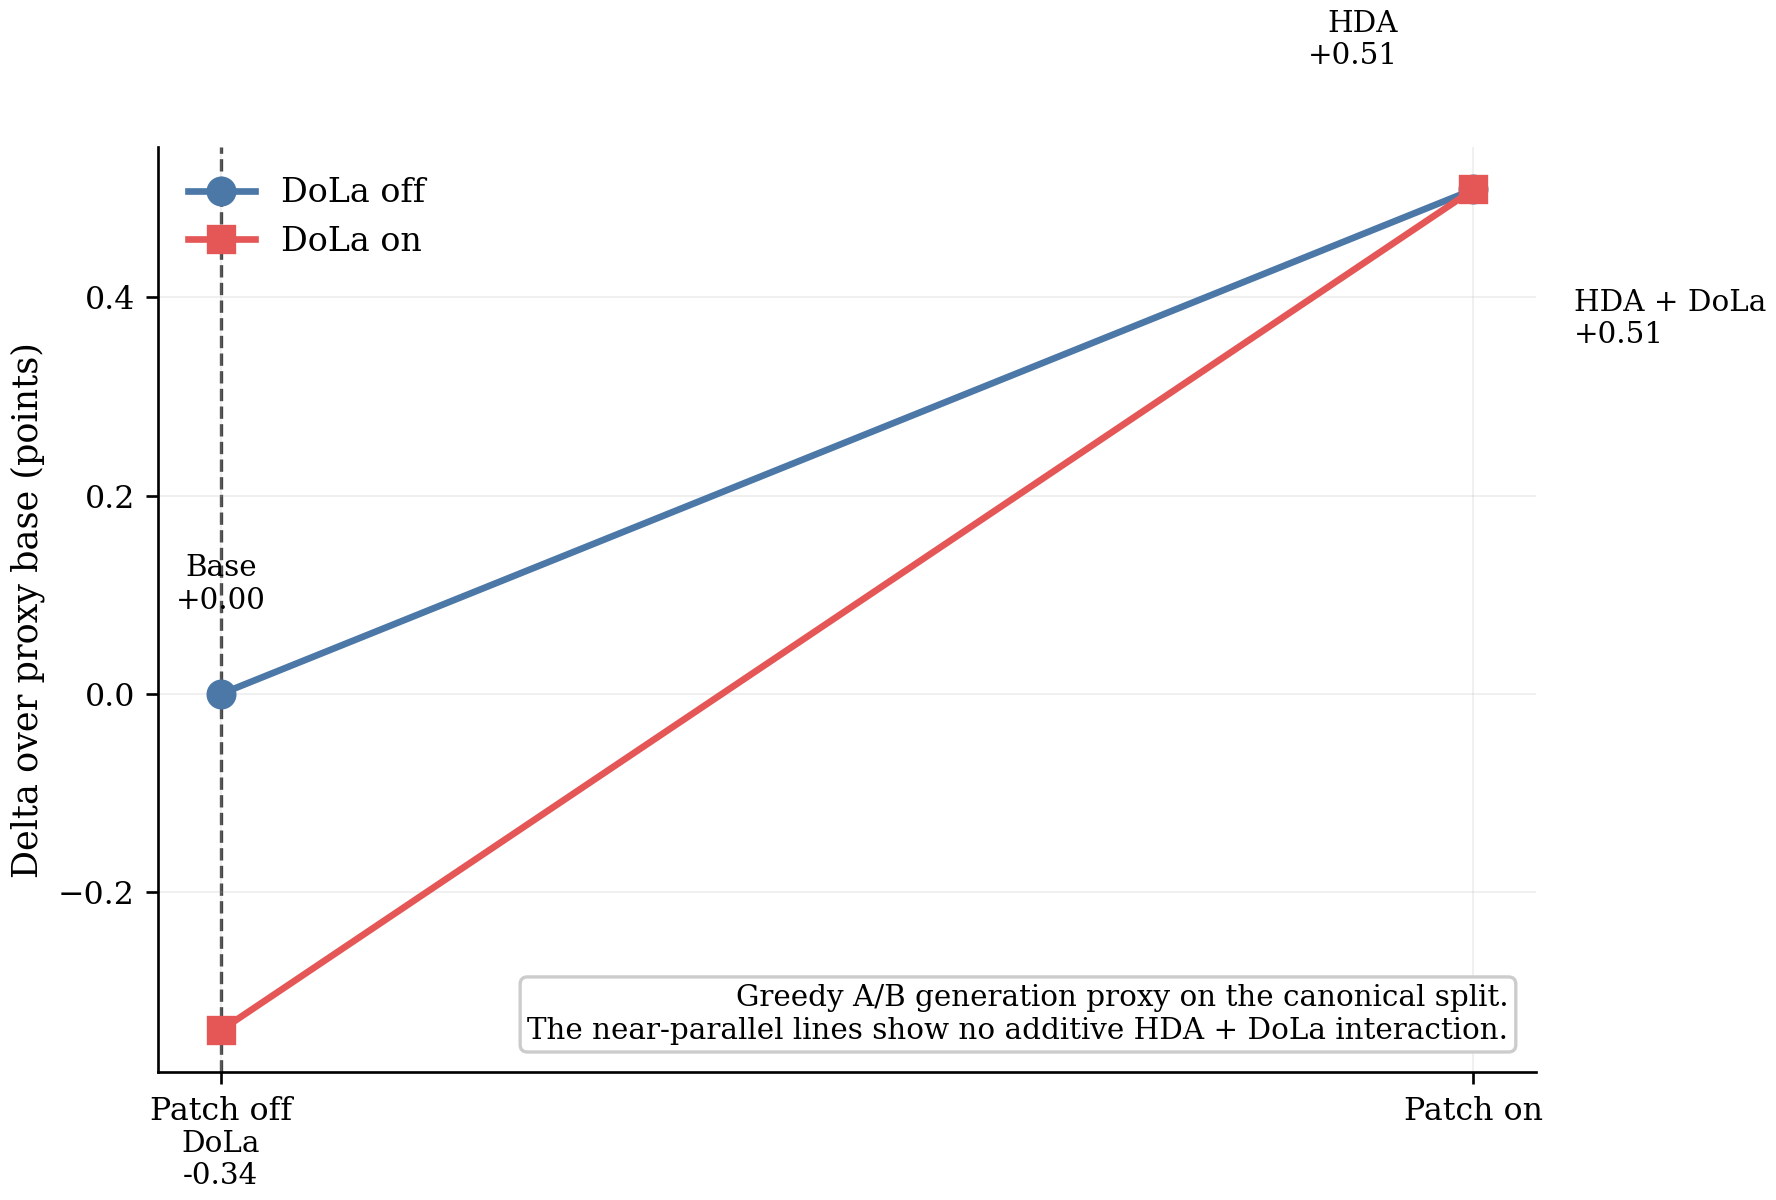
\includegraphics[width=0.88\linewidth]{experiments/artifacts/route_plots/final_qwen4b_dola_proxy.png}
  \caption{DoLa comparison on the Qwen3-4B greedy A/B generation proxy, shown as a $2 \times 2$ interaction plot. This setting is decode-compatible but not directly protocol-equivalent to the main binary log-probability scorer, and it is structurally narrower than DoLa's intended multi-token generation regime.}
  \label{fig:dola-proxy}
\end{figure}

\subsection{Route Pivot: Verifier Reranking Is the Strongest Internal Method}
Although the project began from HDA, the strongest result in the repository is verifier reranking. On the standardized six-seed comparison, the fixed factual verifier prompt improves TruthfulQA by \textbf{+2.37 points over 6 seeds}, with \textbf{6/6 seeds positive}, while the selected-verifier route reaches \textbf{+1.55 points}; the fixed factual variant therefore leads by \textbf{+0.82 points} on the shared seeds. The corresponding two-sided exact sign test for 6/6 positive split deltas is $p=0.03125$. The verifier is not an external model: it is the same base model run through an additional yes/no factuality scoring pass over each candidate answer, using prompts of the form ``Is the candidate answer factually correct? Reply with only yes or no.'' This makes verifier reranking easy to reproduce in the same codebase, but it also means a clear latency tradeoff: unlike the permanent patch, verifier reranking adds extra forward passes at inference time, and we did not run a separate wall-clock latency benchmark here. This route is much stronger than the HDA patch and is the cleanest empirical story for the final presentation. The final interpretation is therefore:
\begin{itemize}
\item \textbf{HDA patch} is the proposal-consistent mechanistic method;
\item \textbf{Verifier reranking} is the best empirical route in the codebase;
\item \textbf{DoLa} is the external prior-method baseline used for comparison.
\end{itemize}
This three-way framing is important because it keeps the presentation honest: the original method works, but another internal route works better.

\subsection{Cross-Model Portability}
The project also tested whether the HDA idea transfers beyond the main 4B model. Results are mixed:
\begin{itemize}
\item \textbf{Qwen3-1.7B}: +0.27 points over 5 seeds after hard non-thinking mode is enabled; no drop on the small regression pack, but the gain is modest.
\item \textbf{Qwen3-0.6B}: +1.02 points over 5 seeds, but GSM8K drops by 4 points and benign drift is noticeably larger.
\item \textbf{Llama-3.2-1B}: +1.29 points over 5 seeds, but GSM8K drops by 3 points on the regression pack.
\end{itemize}
Thus portability exists, but clean portability does not. Only Qwen3-4B currently offers the combination of stable truthfulness gain and no measured collateral regression on the chosen regression pack. Portability should therefore be interpreted as a boundary condition rather than as a central strength of the method.

\begin{figure}[t]
  \centering
  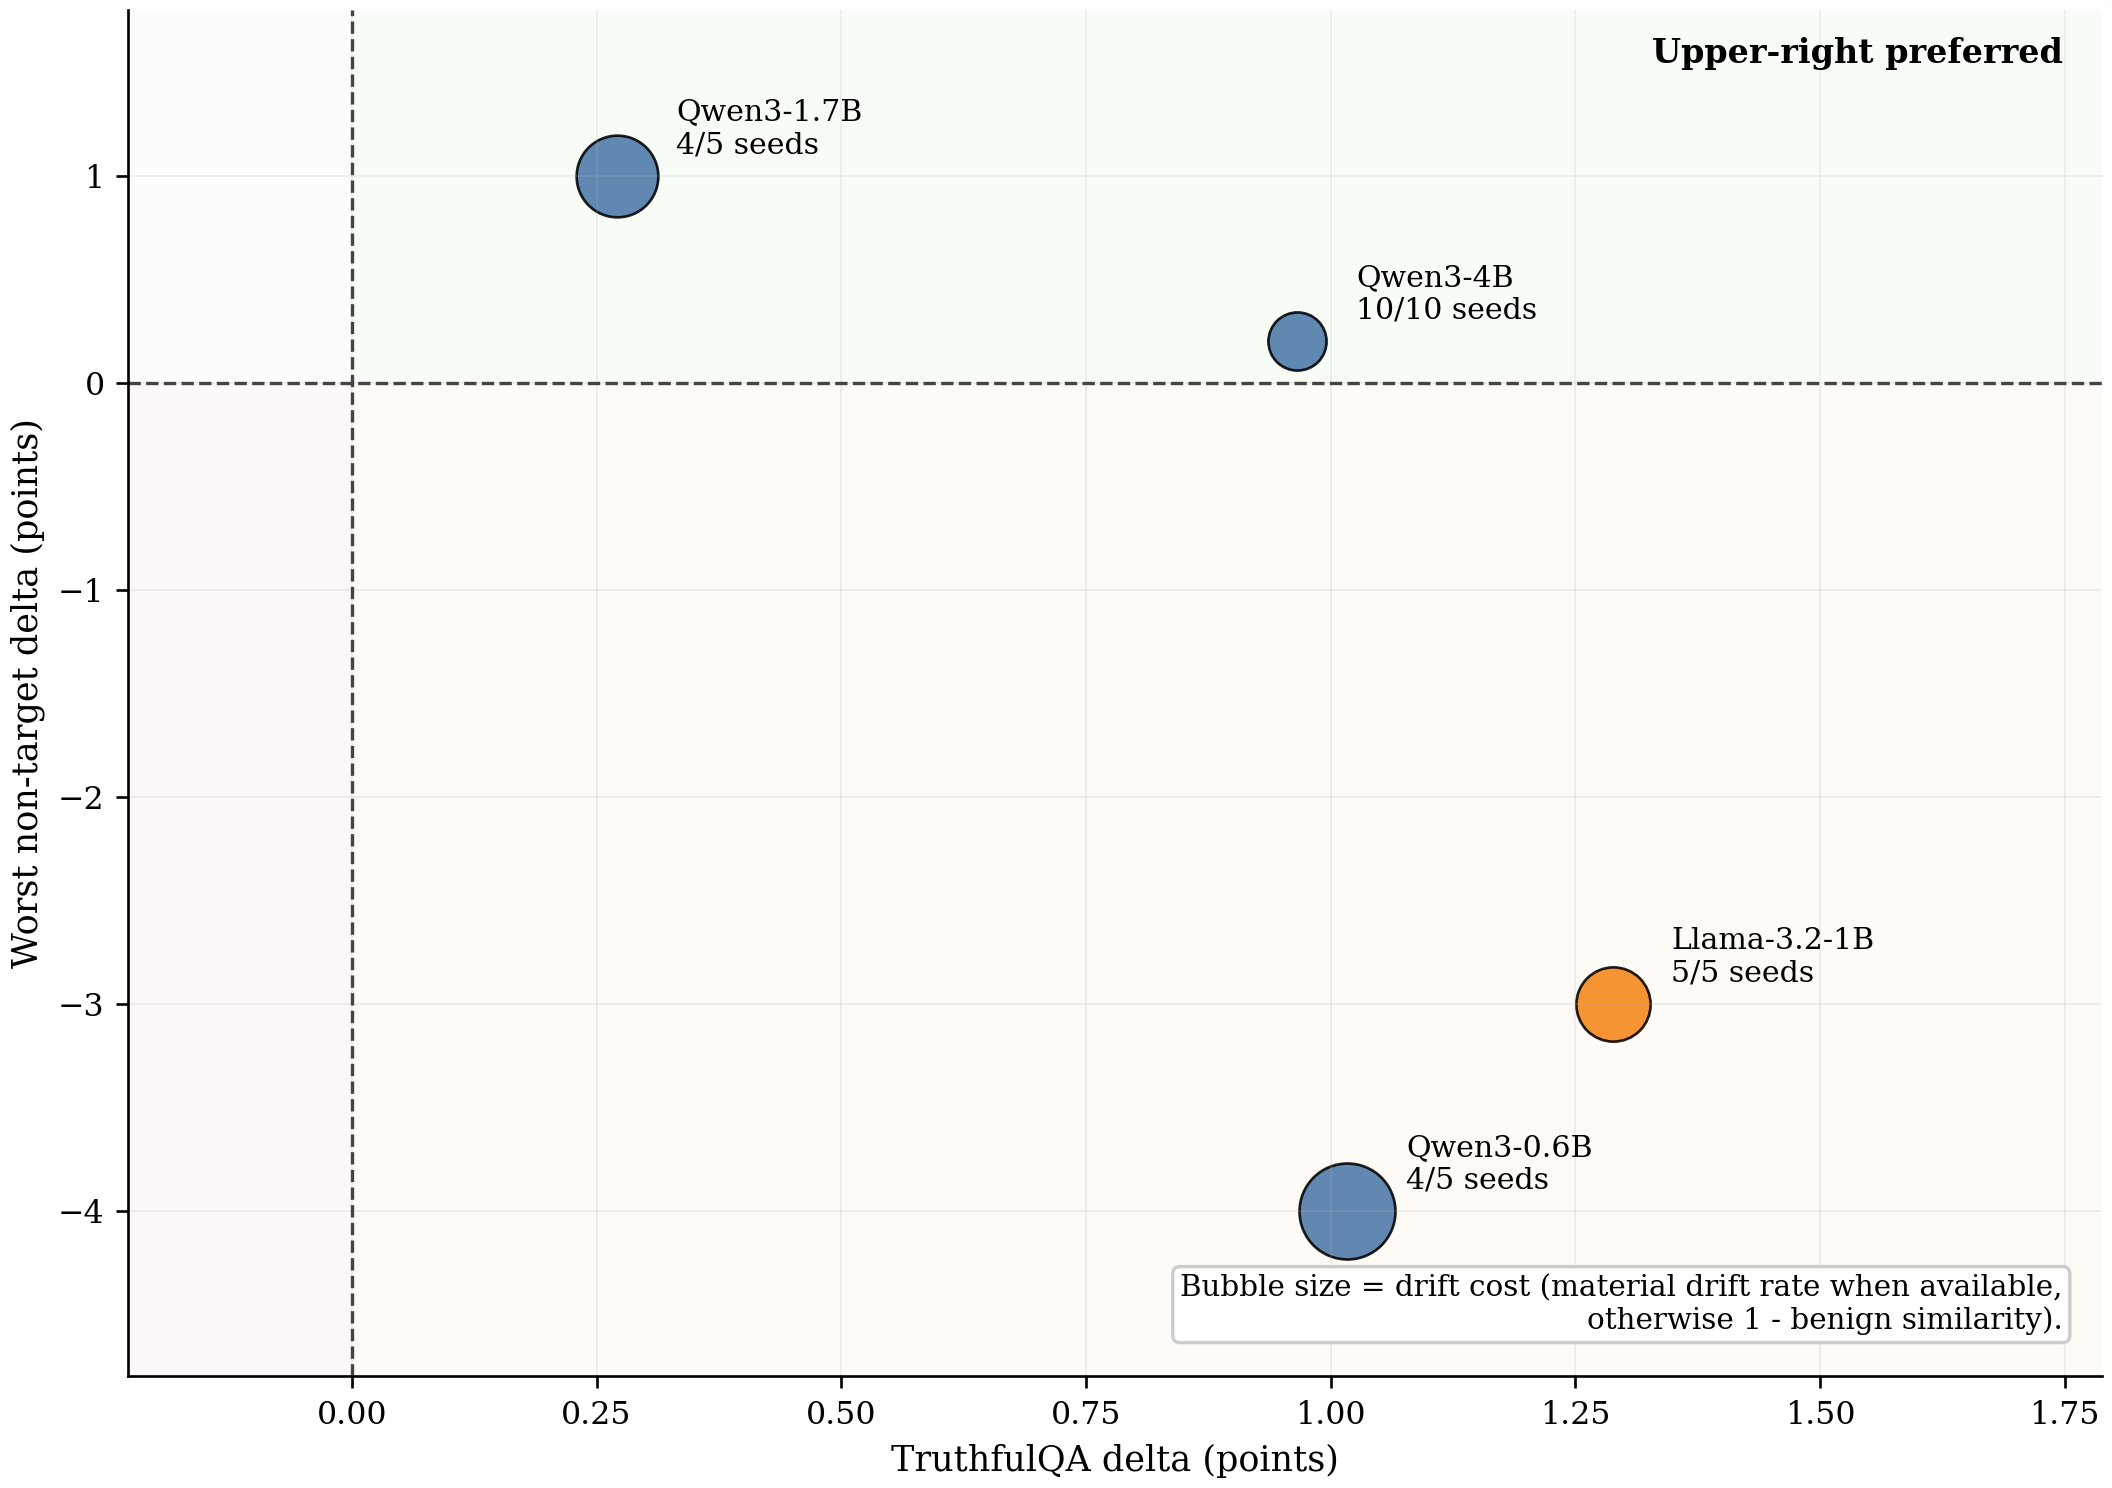
\includegraphics[width=0.9\linewidth]{experiments/artifacts/route_plots/final_cross_model_tradeoff.png}
  \caption{Cross-model portability of HDA patching. Qwen3-4B is the only tested model that improves truthfulness without a measured regression on the lightweight non-target suite.}
  \label{fig:cross-model}
\end{figure}

\subsection{Qwen3 Small Models Require Non-Thinking Mode}
The smaller Qwen3 models initially appeared broken under the binary evaluator because they almost always preferred option \texttt{A}. The cause was not HDA but the default reasoning mode. On a 100-question diagnostic:
\begin{itemize}
\item \textbf{Qwen3-1.7B default}: 48\% accuracy, 100\% A predictions
\item \textbf{Qwen3-1.7B hard no-think}: 65\% accuracy, 39\% A predictions
\item \textbf{Qwen3-0.6B default}: 48\% accuracy, 100\% A predictions
\item \textbf{Qwen3-0.6B hard no-think}: 54\% accuracy, 64\% A predictions
\end{itemize}
This diagnosis mattered scientifically: without it, all downstream patch sweeps on the small Qwen3 models would have been evaluating a degenerate scorer. We interpret this as an evaluator-specific diagnostic for hybrid reasoning models under our binary protocol, not as a broad claim about the models' overall reasoning quality.

\begin{figure}[t]
  \centering
  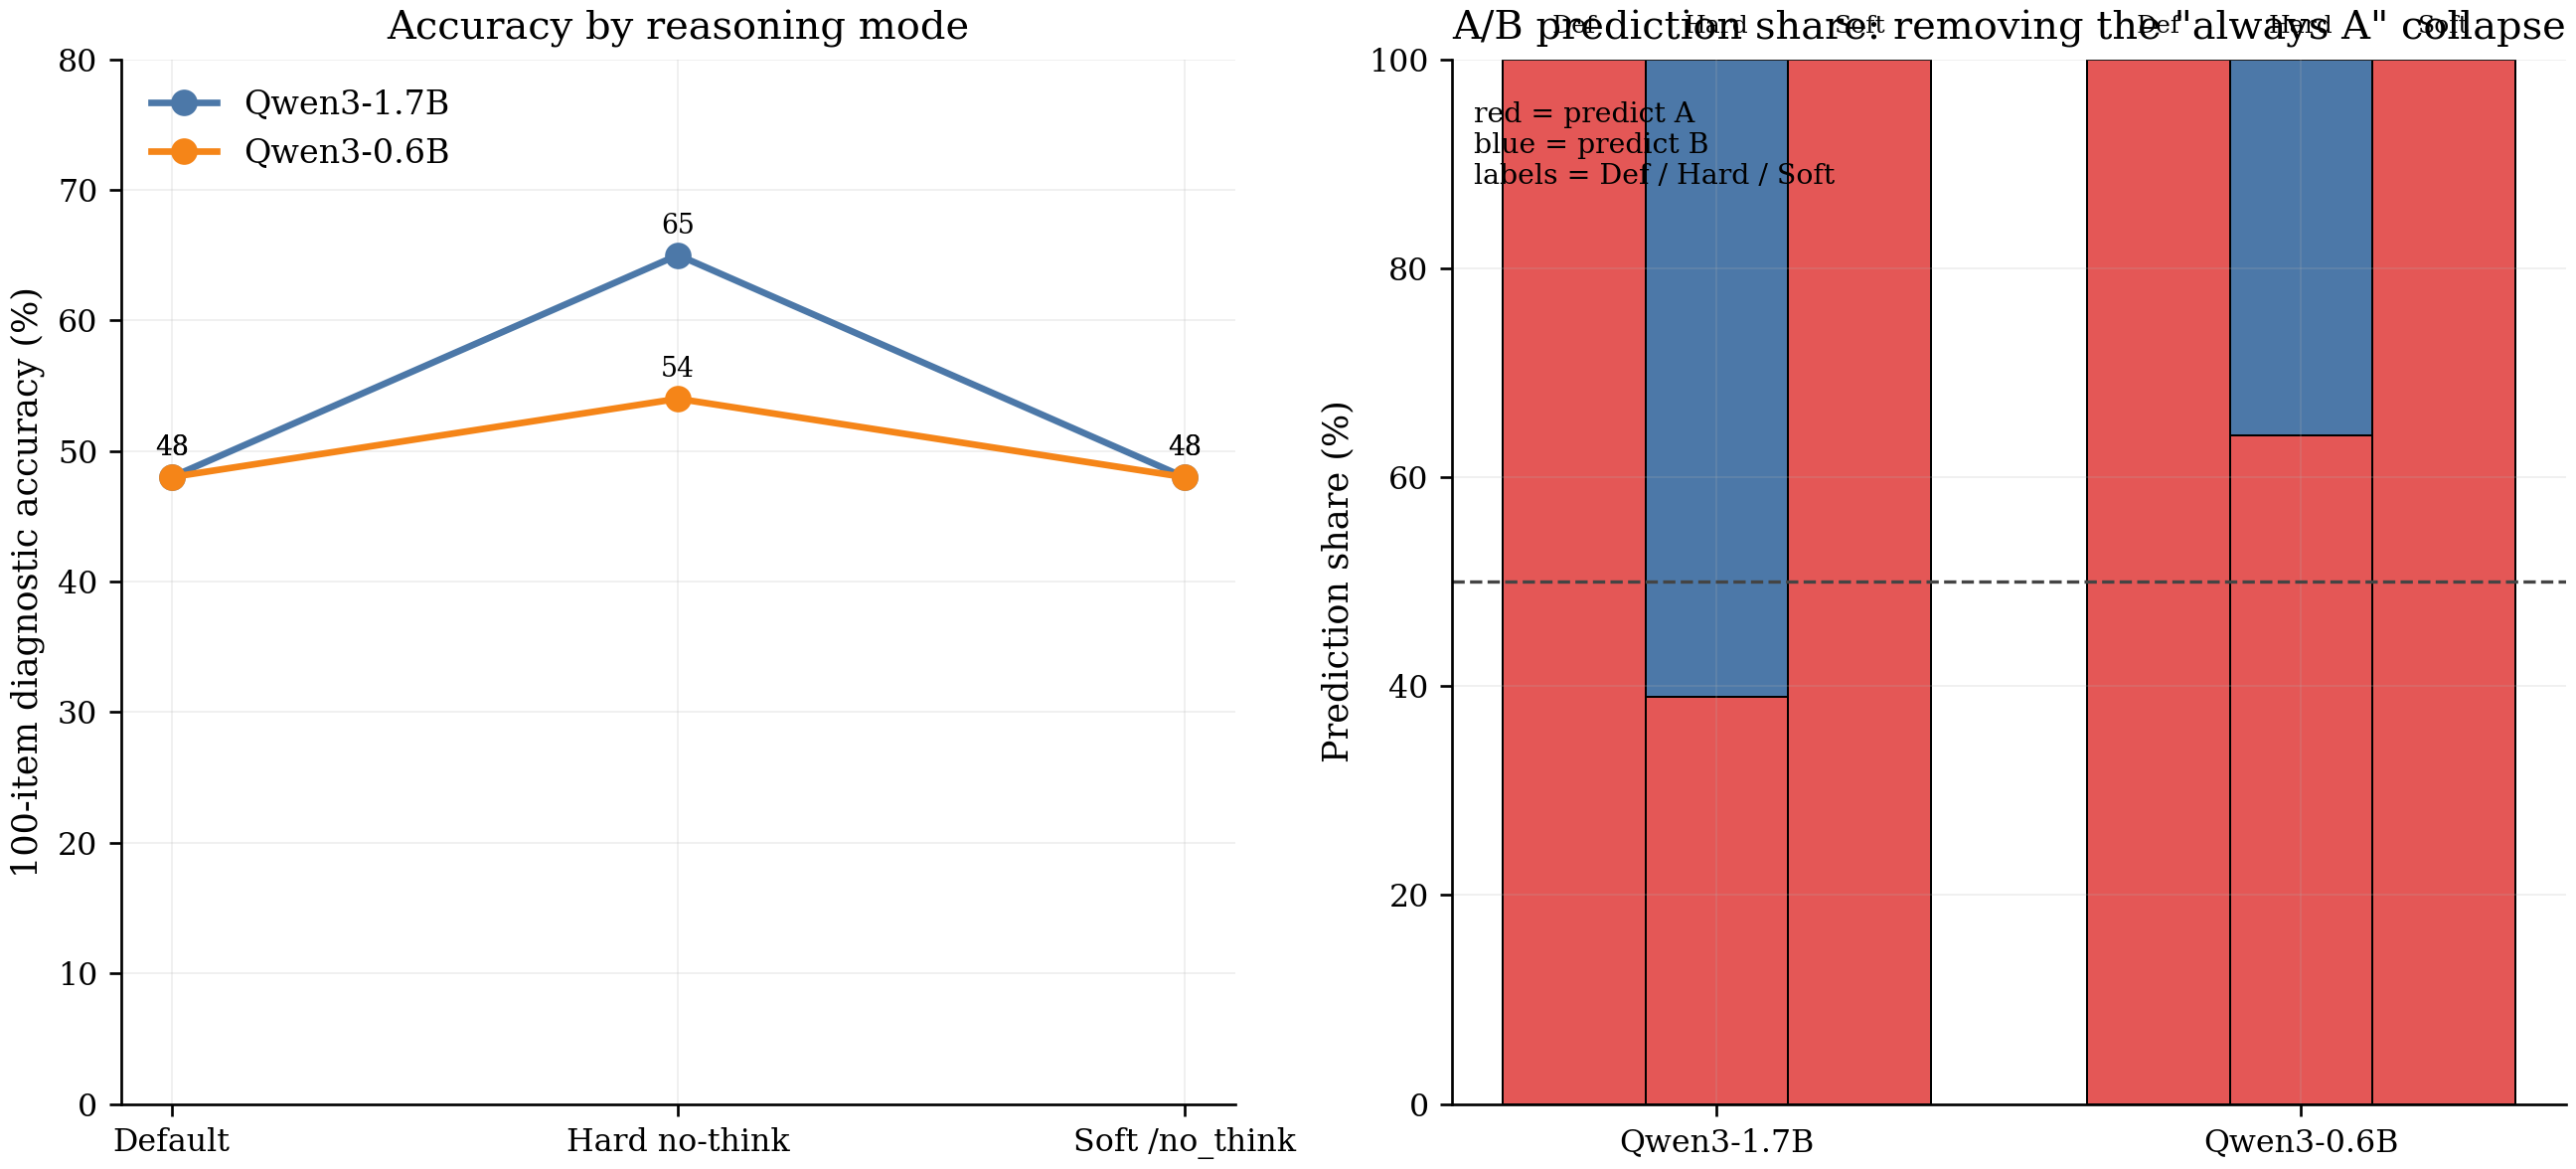
\includegraphics[width=\linewidth]{experiments/artifacts/route_plots/final_qwen_reasoning_diagnosis.png}
  \caption{Reasoning mode diagnosis for Qwen3 small models. Hard-disabling thinking removes the ``always A'' collapse and makes binary evaluation meaningful.}
  \label{fig:qwen-thinking}
\end{figure}

\subsection{Result Synthesis}
The final evidence supports six claims:
\begin{enumerate}
\item HDA patching is \textbf{real but modest}. On Qwen3-4B it gives a stable $\sim$+1 point truthfulness gain, not a dramatic jump.
\item The effect depends on \textbf{where} and \textbf{how strongly} the patch is applied; alpha $=1$ and all-layer patching are clearly weaker than the tuned narrow patch.
\item The regression evidence supports a \textbf{narrow late-MLP family} claim more strongly than a unique exact-band discovery; 18--19 / MLP / $\alpha=2.8$ is kept as the canonical operating point by parsimony.
\item A lightweight paired regression package suggests that the best 4B patch does \textbf{not} buy its gain through obvious measured collateral damage.
\item DoLa does \textbf{not} beat the base model in the project's decode-compatible proxy, and the HDA+DoLa combination does not add to HDA.
\item The strongest empirical route in the repository is verifier reranking, not the permanent patch.
\item The binary gain does \textbf{not} carry over cleanly into open-generation support on the 40-row bridge, so the HDA claim is proxy-limited rather than a validated free-form truthfulness improvement.
\end{enumerate}

\section{Code and Experiment Running Snippets}
The codebase is organized into scripts for data preparation, direction extraction, patching, regression testing, and plotting. Representative commands are shown below.

\paragraph{HDA patch evaluation on Qwen3-4B.}
\begin{verbatim}
python experiments/scripts/weight_patch_eval.py ^
  --model Qwen/Qwen3-4B-Instruct-2507 ^
  --directions experiments/artifacts/directions_qwen4b_cal200_taskaligned.npz ^
  --layers 18,19 --modules mlp --alpha 2.8 ^
  --candidate-prefix newline --seed 41
\end{verbatim}

\paragraph{Regression suite for a fixed patch.}
\begin{verbatim}
python experiments/scripts/run_patch_regression_suite.py ^
  --model Qwen/Qwen3-4B-Instruct-2507 ^
  --directions experiments/artifacts/directions_qwen4b_cal200_taskaligned.npz ^
  --layers 18,19 --modules mlp --alpha 2.8
\end{verbatim}

\paragraph{DoLa-compatible generation proxy.}
\begin{verbatim}
python experiments/scripts/truthfulqa_binary_generate_eval.py ^
  --model Qwen/Qwen3-4B-Instruct-2507 ^
  --dola --dola-layers high
\end{verbatim}

\paragraph{Final figure generation.}
\begin{verbatim}
.venv\Scripts\python.exe experiments/scripts/make_final_project_figures.py
\end{verbatim}

\section{Related Work}
\paragraph{Benchmark and decode-time factuality methods.}
TruthfulQA established the benchmark motivation by showing that large models often imitate human falsehoods rather than answer truthfully \citep{lin-etal-2022-truthfulqa}. DoLa is the most directly relevant external baseline in this report: it is a training-free decode-time factuality method based on contrasting transformer layers during generation \citep{chuang2024dola}. Our comparison differs in intervention location: DoLa changes decoding, whereas HDA changes model parameters once and then uses standard inference.

\paragraph{Sampling-based and inference-time intervention methods.}
SelfCheckGPT represents the sampling-based verification family, which can improve reliability at the cost of repeated generation \citep{manakul-etal-2023-selfcheckgpt}. TruthX is closer in spirit to hidden-state intervention, editing model behavior in a truthful latent space at inference time rather than via a permanent patch \citep{zhang-etal-2024-truthx}. Relative to these methods, our main HDA route aims for a permanent, training-free edit with no additional runtime controller.

\paragraph{Permanent editing and mechanistic direction-control.}
ROME and related knowledge-editing methods motivate permanent parameter editing, although their main focus is fact-specific editing rather than global hallucination suppression \citep{meng2022rome}. Inference-Time Intervention and recent work on refusal directions both support the broader idea that low-dimensional directions can be used as intervention targets \citep{li2024iti,arditi2024refusal}. Practical tooling such as Heretic also demonstrates that direction-based ablation can be turned into an operational steering pipeline \citep{weidmann2025heretic}. Our HDA route is most closely aligned with this last family, but is evaluated here specifically as a TruthfulQA truthfulness intervention rather than as a general-purpose steering framework.

Relative to these lines, this project contributes a compact, end-to-end experimental answer to a practical question: how far can a training-free \emph{permanent} patch go on truthfulness before regression becomes unacceptable, and how does it compare to a decode-time baseline and a verifier pivot?

\section{Conclusion}
The final answer is nuanced but useful. The original HDA idea works: a carefully placed training-free directional patch can improve truthfulness on Qwen3-4B, and the gain is stable across 10 seeds. However, the effect is small, and the original ``alpha $=1$ everywhere'' intuition is not enough. The effective patch is stronger and narrower, and its geometric role is better described as tuned over-subtractive suppression than as a pristine projector. The evidence is strongest for a narrow late-MLP family, with layers 18--19 / MLP / $\alpha=2.8$ kept as the canonical operating point by parsimony rather than by a decisive exact-band win over the neighboring 18--20 setting.

The strongest practical route in this project is verifier reranking, not the permanent patch. This matters for the final presentation because it lets the project tell a complete story: the proposal-consistent mechanistic method achieves a real and interpretable gain; a stronger internal route emerges during experimentation; and a recognized external baseline (DoLa) does not surpass the project's best patch under the decode-compatible proxy.

The most defensible final claim is therefore not that HDA is the universally best hallucination solution. It is that \textbf{a carefully placed permanent patch can produce a reproducible, modest truthfulness gain on the main model under a lightweight regression audit}, while stronger gains in this codebase currently come from verifier reranking. More precisely, the best-performing version of the method should be read as a tuned suppressive directional patch derived from an orthogonal-projection starting point, not as a pure orthogonal projector. The method remains viable and lightweight, but its benefit is modest, its portability is only partial, its main evidence comes from a ranking-style binary proxy rather than from full free-form generation, and the binary-to-open bridge in this project did \emph{not} show stronger open-generation support for the patched model. That bridge result pushes the final HDA claim down to \textbf{proxy-limited evidence}: useful, repeatable, and practically interesting, but not yet validated as a broader open-ended hallucination fix.

\begin{thebibliography}{9}

\bibitem[Arditi et~al.(2024)]{arditi2024refusal}
Andy Arditi, Oscar Obeso, Aaquib Syed, Daniel Paleka, Nina Panickssery, Wes Gurnee, and Neel Nanda.
\newblock Refusal in Language Models Is Mediated by a Single Direction.
\newblock \emph{arXiv preprint arXiv:2406.11717}, 2024.

\bibitem[Chuang et~al.(2024)]{chuang2024dola}
Yung-Sung Chuang, Yujia Xie, Hongyin Luo, Yoon Kim, James R. Glass, and Pengcheng He.
\newblock DoLa: Decoding by Contrasting Layers Improves Factuality in Large Language Models.
\newblock In \emph{The Twelfth International Conference on Learning Representations}, 2024.

\bibitem[Li et~al.(2024)]{li2024iti}
Kenneth Li, Oam Patel, Fernanda Vi{\'e}gas, Hanspeter Pfister, and Martin Wattenberg.
\newblock Inference-Time Intervention: Eliciting Truthful Answers from a Language Model.
\newblock \emph{arXiv preprint arXiv:2306.03341}, 2024.

\bibitem[Lin et~al.(2022)]{lin-etal-2022-truthfulqa}
Stephanie Lin, Jacob Hilton, and Owain Evans.
\newblock TruthfulQA: Measuring How Models Mimic Human Falsehoods.
\newblock In \emph{Proceedings of the 60th Annual Meeting of the Association for Computational Linguistics (Volume 1: Long Papers)}, pages 3214--3252, 2022.

\bibitem[Manakul et~al.(2023)]{manakul-etal-2023-selfcheckgpt}
Potsawee Manakul, Adian Liusie, and Mark Gales.
\newblock SelfCheckGPT: Zero-Resource Black-Box Hallucination Detection for Generative Large Language Models.
\newblock In \emph{Proceedings of the 2023 Conference on Empirical Methods in Natural Language Processing}, pages 9004--9017, 2023.

\bibitem[Meng et~al.(2022)]{meng2022rome}
Kevin Meng, David Bau, Alex Andonian, and Yonatan Belinkov.
\newblock Locating and Editing Factual Associations in GPT.
\newblock In \emph{Advances in Neural Information Processing Systems}, 2022.

\bibitem[Weidmann(2025)]{weidmann2025heretic}
Philipp Emanuel Weidmann.
\newblock Heretic: Fully Automatic Censorship Removal for Language Models.
\newblock GitHub repository, 2025.

\bibitem[Zhang et~al.(2024)]{zhang-etal-2024-truthx}
Shaolei Zhang, Tian Yu, and Yang Feng.
\newblock TruthX: Alleviating Hallucinations by Editing Large Language Models in Truthful Space.
\newblock In \emph{Proceedings of the 62nd Annual Meeting of the Association for Computational Linguistics (Volume 1: Long Papers)}, pages 8908--8949, 2024.

\end{thebibliography}

\end{document}
